\documentclass{article}
% translate with >> pdflatex -shell-escape <file>

% This file is used as unit test for pgfplots, copyright by Christian Feuersaenger.
% 
% See
%   http://pgfplots.sourceforge.net/pgfplots.pdf
% for pgfplots.
%
% Any required input files (for <plot table> or <plot file> or the table package) can be downloaded
% at
% http://www.ctan.org/tex-archive/graphics/pgf/contrib/pgfplots/doc/latex/
% and
% http://www.ctan.org/tex-archive/graphics/pgf/contrib/pgfplots/doc/latex/plotdata/

\usepackage{pgfplots}
\pgfplotsset{compat=newest}

\pagestyle{empty}

\begin{document}
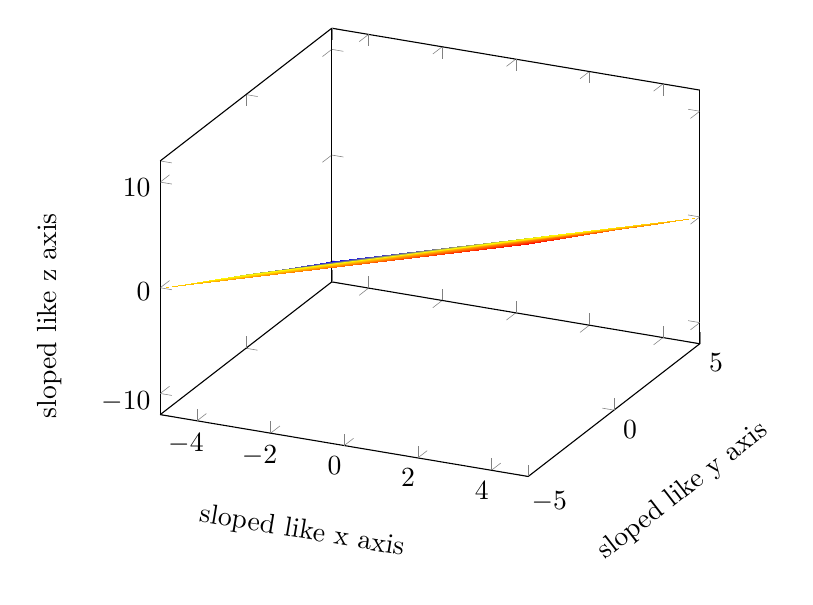
\begin{tikzpicture}
	\begin{axis}[samples=5,
		extra description/.append code={%
			\node[sloped like x axis] at (xticklabel cs:0.5,15pt) {sloped like x axis};
			\node[sloped like y axis] at (yticklabel cs:0.5,15pt) {sloped like y axis};
			\node[sloped like z axis] at (zticklabel cs:0.5,15pt) {sloped like z axis};
		},
	]
	\addplot3[surf,shader=interp] {x-y};
	\end{axis}
\end{tikzpicture}
\end{document}
